\documentclass[UTF8]{ctexart}
\usepackage{amsmath,amssymb}
\usepackage{fancyhdr}
\usepackage{amsmath,bm}
\usepackage{mathrsfs}
\usepackage{ntheorem}
\usepackage{graphicx}
\usepackage{subfigure}
\usepackage[top=2cm, bottom=2cm, left=2cm, right=2cm]{geometry}  
\usepackage{algorithm}  
\usepackage{algorithmicx}  
\usepackage{algpseudocode}
\usepackage{tikz}
\usetikzlibrary{automata, positioning, arrows}
\tikzset{
    ->,
    >=stealth,
    node distance = 3cm,
    every state/.style={thick, fill=gray!10},
    initial text=$ $
}

\floatname{algorithm}{算法}  
\renewcommand{\algorithmicrequire}{\textbf{输入:}}  
\renewcommand{\algorithmicensure}{\textbf{输出:}}  
  
\theorembodyfont{\normalfont\rm\CJKfamily{song}}
%\theoremstyle{break}
\newtheorem{theorem}{定理}
\newtheorem{lemma}{引理}
\newtheorem{proposition}{命题}
\newtheorem*{proof}{证}[section]
\newtheorem*{solution}{解}[section]
\title{词法分析作业}
\author{丁元杰 17231164}
\date{\today}

\begin{document}
\maketitle

\section*{3.1}
状态图如图\ref{3_1FSM}
\subsection*{(1)}

\begin{figure}[ht] % ’ht’ tells LaTeX to place the figure ’here’ or at the top of the page
    \centering % centers the figure
    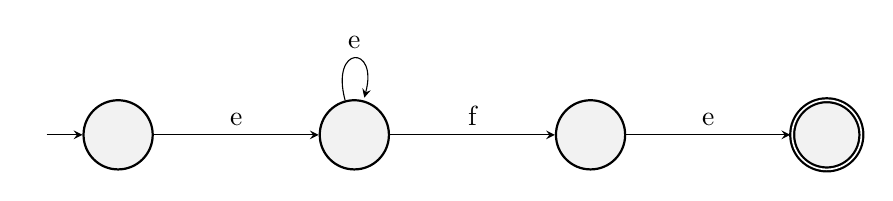
\begin{tikzpicture}
    % tikz code goes here
        \node[state, initial] (q1) { };
        \node[state, right of=q1] (q2) { };
        \node[state, right of=q2] (q3) { };
        \node[state, accepting, right of=q3] (q4) { };
        \draw (q2) edge[loop above] node{e} (q1)
        (q1) edge[above] node{e} (q2)
        (q2) edge[above] node{f} (q3)
        (q3) edge[above] node{e} (q4);
    \end{tikzpicture}
    \caption{3.1 状态图}
    \label{3_1FSM}
\end{figure}
\subsection*{(2)}
可以看出:
\begin{itemize}
    \item $eefe$符合文法
    \item $f$,$eeff$不符合文法
\end{itemize}

\section*{3.2}
\subsection*{(1)}
文法如下:
\begin{align*}
    <S>&::=0\ \big| \ 0A \\
    <A>&::=1\ \big|\ 0A
\end{align*}

\subsection*{(2)}
$$V=\{0, 1, S, A\}$$
$$V_t=\{0, 1\}$$
$$V_n=\{S, A\}$$

\subsection*{(3)}
$$L(G)=\{0, 0^n1 \big|n\in\mathbb N^*\}$$

\end{document}